\section{Introduction to Thermodynamics}
\textit{Note: The following gives a brief overview of thermodynamics. The specific details will be covered in more depth.}
\begin{itemize}
    \item The major idea of this course is developing methods to create efficient heat engines to do useful work.
          \begin{example}
              In a \textbf{Newcomen Engine,} there are two valves. By alternating the states of each valve, it is possible to move the piston up and down (around 5 times a minute).
              \begin{center}
                  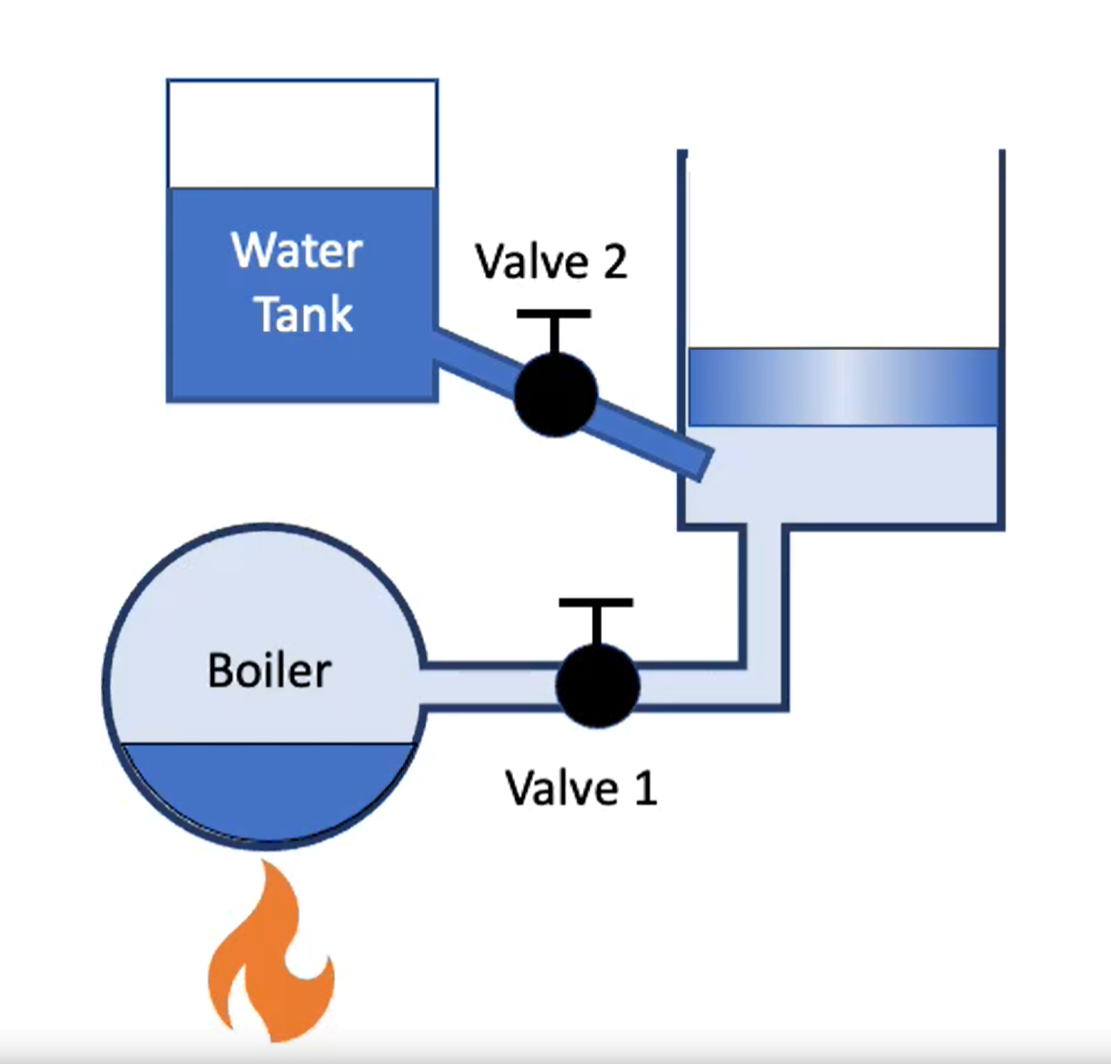
\includegraphics[width=0.4\linewidth]{L01-Newcomen.png}
              \end{center}
              When Valve 1 opens, steam fills the chamber and lifts up the piston. When Valve 2 opens (with valve 1 closes), water gets sprayed, evaporates, and condenses, causing the piston to lower.
              \vspace{2mm}

              Unfortunately, this is very inefficient as the majority of the energy goes into heating and cooling the water, instead of actually moving the piston.
          \end{example}
    \item The steam engine can be improved using the \textbf{Watt Engine} design. Instead of having a water tank, a condenser is used. When Valve 2 opens, the steam exits into a condenser which then gets turned to water.
    \item The steam cycle can be illustrated below.
          \begin{center}
              \begin{tikzpicture}
                  \begin{scope}[xshift=0cm,yshift=0cm]
                      \node (boiler) [process] at (2,2) {Boiler};
                      \node (turbine) [process] at (4, 0) {Turbine};
                      \node (condenser) [process] at (2,-2) {Condenser};
                      \node (pump) [process] at (0, 0) {Pump};

                      \draw[-latex] (boiler.east) -> (turbine.north);
                      \draw[-latex] (turbine.south) -> (condenser.east);
                      \draw[-latex] (condenser.west) -> (pump.south);
                      \draw[-latex] (pump.north) -> (boiler.west);
                  \end{scope}
              \end{tikzpicture}
          \end{center}
          \begin{definition}
              A heat engine is anything that takes heat and does useful work.
          \end{definition}
    \item A heat engine has a high temperature heat source, a low temperature heat sink, and performs useful work.
    \begin{center}
        \begin{tikzpicture}
            \node (heat engine) [process] at (0,0) {Heat Engine};
            \node (heat source) [process] at (0,2) {Heat Source \\ High Temperature $T_H$};
            \node (heat sink) [process] at (0,-2) {Heat Sink \\ Low Temperature $T_C$};
            \node (work) [process] at (4,0) {Work};

            \draw[-latex] (heat source.south) -> (heat engine.north) node[midway,right] {Heat input $Q_H$};
            \draw[-latex] (heat engine.south) -> (heat sink.north) node[midway,right] {Heat rejected $Q_C$};
            \draw[-latex] (heat engine.east) -> (work.west);
        \end{tikzpicture}
    \end{center}
    Note that by useful work, we refer to the ability to apply a force over a distance (i.e. lift up a box).
    \item The \textbf{First Law of Thermodynamics} is the conservation of energy.
    \begin{idea}
        At steady state, the energy added as heat must equal the energy removed as work. In other words, 
        \begin{equation}
            W = Q_H - Q_C
        \end{equation}
    \end{idea}
    \item We can define the thermal efficiency to be
    \begin{equation}
        \eta_{th} = \frac{\text{Net work output}}{\text{Heat input}} = \frac{W}{Q_H} = \frac{Q_H-Q_C}{Q_H}
    \end{equation}
    or
    \begin{equation}
        \eta_\text{th} = 1 - \frac{Q_C}{Q_H}
    \end{equation}
    \item For context:
    \begin{itemize}
        \item Newcommen Engine $\eta_\text{th} =0.34\%$
        \item Watt Engine 1770 $\eta_\text{th} = 4\%$
        \item Watt Engine 1850 $\eta_\text{th} = 15\%$
        \item Modern Steam Power Plant $\eta_\text{th}=30-35\%$
    \end{itemize}
    \item Note that the wasted energy is going into $Q_C$. Is it possible for $Q_C=0$? The answer is no.
    \item Every system has a property called \textbf{entropy}. Entropy of a system changes when there is a heat transfer to or from it. The change in entropy can be defined as:
    \begin{equation}
        \Delta S = \frac{\text{heat transferred}}{\text{temperature}} = \frac{Q_H}{T_H}
    \end{equation}
    \begin{idea}
        In a reversible process (we will learn more about this later), the entropy into a system is equal to the entropy that gets transferred out of a system.
    \end{idea}
    Applying this idea, we get
    \begin{equation}
        \frac{\Delta S_\text{in}}{\Delta S_\text{out}} = \frac{Q_H}{T_H} = \frac{Q_C}{T_C}
    \end{equation}
    Rearranging and substituting this into the formula for efficiency, we get
    \begin{equation}
        \eta_\text{th} = 1 - \frac{T_C}{T_H}
    \end{equation}
    This can only reach $100\%$ if $T_C=0$, which is impossible.
\end{itemize}
